\begin{center}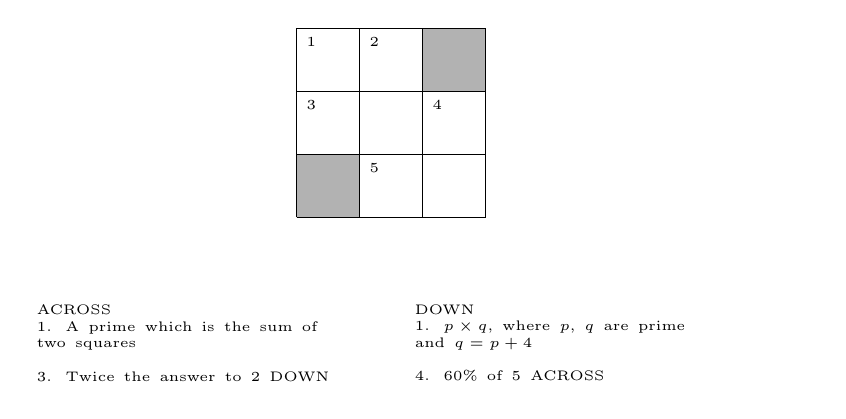
\begin{tikzpicture}[scale = .8]
\fill[black!30](0,0)rectangle(1,1) (2,2)rectangle(3,3);
\draw(0,0)grid(3,3);
\node[below right] at(0,3) {\tiny $1$};
\node[below right] at(0,2) {\tiny $3$};
\node[below right] at(1,3) {\tiny $2$};
\node[below right] at(2,2) {\tiny $4$};
\node[below right] at(1,1) {\tiny $5$};
\node[text width = 5cm] at(-1,-2){\tiny ACROSS \\ 1. A prime which is the sum of\\two squares\\3. Twice the answer to 2 DOWN};
\node[text width = 5cm] at(5,-2){\tiny DOWN \\ 1. $p\times q$, where $p$, $q$ are prime \\and $q = p + 4$\\4. $60\%$ of 5 ACROSS};
\end{tikzpicture}\end{center}
